\documentclass[10pt,oneside,a4paper,final,english]{memoir}

\usepackage{palatino}
\usepackage{microtype}
\usepackage{lscape}
\usepackage{multicol}
%\usepackage{epic,eepic}
\usepackage{latexsym}
\usepackage{verbatim}
\usepackage{listings}
\usepackage{ulem}
\usepackage{hyperref}

\let\footruleskip\undefined
\usepackage{fancyhdr}
\usepackage[final]{fixme}

\let\fref\undefined
\usepackage[plain]{fancyref}

%% FOR LOOP
\usepackage{ifthen,calc}
\newcounter{myforloopcounter}
\newcommand{\forloop}[5][1]% 
{\setcounter{#2}{#3}% 
\ifthenelse{#4}% 
{#5%
  \addtocounter{#2}{#1}% 
  \forloop[#1]{#2}{\value{#2}}{#4}{#5}% 
}%
% Else 
{}%
}% 


%% USAGE
%\forloop[step]{counter}{initial_value}{conditional}{code_block} 
\usepackage[english]{babel}
\usepackage[utf8]{inputenc}

%\selectlanguage{danish}

\lstset{language=Python,basicstyle=\small,
  columns=fullflexible}


\usepackage[pdftex]{graphicx}

\DeclareGraphicsExtensions{.jpg .png .pdf}


\usepackage{amsmath}
\usepackage{latexsym}
\usepackage{amssymb}


\usepackage[osf,sc]{mathpazo}
\usepackage{microtype}
%\usepackage{fourier}
\linespread{1.05}

%\usepackage[charter]{mathdesign}
%\usepackage{lmodern}

%\usepackage{algorithmic}
%\usepackage{algorithm}

\usepackage{amsthm}


\theoremstyle{plain}  \newtheorem{definition}{Definition}
\theoremstyle{remark} \newtheorem{lemma}{Lemma}
\theoremstyle{plain}  \newtheorem{theorem}{Theorem}
\theoremstyle{remark}  \newtheorem{example}{Example}


\newcommand{\p}{\ensuremath{^\prime}}
\DeclareGraphicsExtensions{.jpg, .eps, .png}
%%% Local Variables:
%%% mode: plain-tex
%%% TeX-master: "../master"
%%% End:

\usepackage{algorithmic}
\usepackage{algorithm}
\usepackage[sectionbib,square]{natbib}
%\bibpunct{(}{)}{,}{a}{}{}
\setcitestyle{alpha}
%\setcitestyle{numbers,aysep={},yysep={;}}

\usepackage{datetime}

\chapterstyle{thatcher}

\setcounter{secnumdepth}{0}
\setcounter{tocdepth}{0}




%\pagestyle{fancy}
\begin{document}
  \fontencoding{T1}
%  \fontseries{m}
%  \fontshape{n}
%  \fontsize{12}{15}
%  \selectfont


%%%%%%%%%%%%%%%%%%%%%%%%%%%%%%%%%%%%%%%%%%%%%%%%%%%%%%%%
%                    Forside
%%%%%%%%%%%%%%%%%%%%%%%%%%%%%%%%%%%%%%%%%%%%%%%%%%%%%%%%
\makeatletter % open mode for reading @ signed variables
\def\maketitle{%
 \null
 \thispagestyle{empty}%
 \vfill
 \begin{center}\leavevmode
   \normalfont
   \LARGE{\raggedleft \@title\par}%
   \hrulefill\par
   \large{\raggedleft \subtitle\par}%
   \vskip 2cm
   {\today\par}%
 \end{center}%
 \vfill
 \begin{flushleft}
   {\large \@author } \\
   {\footnotesize \suplementInfo }
 \end{flushleft}
 \clearpage % Terminates the page here. Everything else vil be placed
            % on next page.
}
\makeatother % closing mode for reading @ signed variables
%%%%%%%%%%%%%%%%%%%%%%%%%%%%%%%%%%%%%%%%%%%%%%%%%%%%%%%%
%               Data til forside
%%%%%%%%%%%%%%%%%%%%%%%%%%%%%%%%%%%%%%%%%%%%%%%%%%%%%%%%
\title{Final Hand In $\cdot$ Week VIII}

\def\subtitle{CCO $\cdot$ Constraint Continuous Optimization}

\author{Johan Sejr Brinch Nielsen} \def\suplementInfo{

\kern 5pt \hrule width 11pc \kern 5pt

\begin{tabular}{ll}
Email: & zerrez@diku.dk  \\
Cpr.:  & 260886-2547
\end{tabular}

% putter 5pt spacing oven over og neden under stregen
\kern 5pt \hrule width 11pc \kern 5pt

Dept. of Computer Science,  \\
University of Copenhagen

}


\maketitle
\newpage

\section{Introduction}
The goal of this assignment was to implement the BFGS Quasi-Newton
method and compare this to the two methods implemented so far.

\section{Quasi-Newton Methods}
Many line search methods fall into a group, that can be identified by
a direction computation that takes the following form:
\[ p_{k+1} = - B^{-1} \nabla f(x) \]

Where $B$ is a positive definite matrix and $p_{k+1}$ is the
next search direction. This group of search methods include steepest
descent (with $B = I$) and Newton's method (with $B = \nabla f(x)$).

Quasi-Newton methods are a specific sort of line search methods that
fall into this group. They work like Newton's method, but instead of
using the Hessian, these methods approximate either this or its
inverse directly. The direction $p_k$ is hence computed as either:
\[ p_{k+1} = - B^{-1} \nabla f(x) \]
or \[ p_{k+1} = - Bi \nabla f(x) \]
Where $B$ and $Bi$ are an approximation of the Hessian and its inverse
respectively.

The new direction is now used to update the current solution by:
\[ x_{k+1} = x_k + \alpha p_{k+1} \]
Where $\alpha$ is an appropriately chosen step length.

Quasi-Newton methods may use more iterations than those, who compute
the hessian and its inverse, however each iteration costs much less in
computation time due to the approximations.

\section{Armijo Backtracking}

To figure out when a step length can be considered a \textit{good}
choice, some restrictions on the resulting point has been
suggested. One of these are the Armijo condition. The Armijo condition
states that the function value in the new point should be no more than
that of the tangent of the current point (relaxed by some
constant). This condition is formalized as:
\[ f(x_k + \alpha_k p_k) \leq f(x_k) +
\alpha_k c_1 p_k^T \nabla f(x_k) \]

Where $\alpha_k$ is the current step length, $c_1$ is a constant
relaxing the condition (by raising the gradient of the limiting line)
and $p_k$ is the current search direction.

Armijo backtracking is a simple method for finding a point, that meet
the Armijo condition (hence the name). The algorithm starts with a
large step length (e.g. 1). The step length is then lowered until a
point that meets the condition is found.

If the function is descending in the chosen search direction (which is
assumed) such a point must necessarily exist. However, it may be very
close to the initial $x$. If so, the step taken can be very short,
perhaps nearly nothing at all. Therefore it is important to ensure a
minimum step size.

The algorithm can be described with the following pseudo code:
\begin{verbatim}
while not (Armijo-condition of (x+a pk)) do
  a = a * c1
end
\end{verbatim}


\section{BFGS Method}
The Broyden–Fletcher–Goldfarb–Shanno method (BFGS) is a Quasi-Newton
method. As so it approximates the inverse of the hessian. This
approximation $B_k$ is updated in each iteration like so:
\[ B_{k+1} = B_k + U_k + V_k \]

Where $U_k$ and $V_k$ are update matrices. Let $y_k$ be specified by:
\[ y_k = \nabla f(x_k + \alpha p_k) - \nabla f(x_k) \]

The two update matrices $U_k$ and $V_k$ can now be described as:
\[ U_k = \frac{y_ky_k^T}{y_k^Tp_k} \]
\[ V_k = \frac{B_kp_k(B_kp_k)^T}{p_k^TB_kp_k} \]

These matrices can be used to update the approximation of the hessian,
however in my implementation I approximate the inverse of the hessian
and hence use two slightly different matrices:
\[ U_k' = \frac{(p_kp_k^T) (p_k^Ty_k + y_k^TB_k^{-1}y_k}{(p_k^Ty_k)^2} \]
\[ V_k' = - \frac{B^{-1}y_kp_k^T + p_ky_k^TB_k^{-1}}{p_k^Ty_k} \]

The update step of the approximation of the inverse hessian now
becomes:
\[ B^{-1}_{k+1} = B^{-1}_k + U'_k + V'_k \]

The implementation uses the identity matrix as the initial
approximation.


\section{Implementation}
This section contains the MatLab code for the BFGS implementation. I
also updated the source code for the other two methods slightly,
however I considered the changes too small to include here.

\subsection{Armijo Backtracking}
\verbatiminput{../code/armijo_backtrack.m}
\subsection{BFGS}
\verbatiminput{../code/bfgs.m}


\section{Verification}
In this section I compare the performance of the three algorithms
(Nonlinear Newton's Method, Levenberg Marquardt and BFGS).

I apologize for the small graphs, but MatLab generates white margins
around the graphs and ImageMagick cannot remove them without
destroying the vector format. However, since the graphs are in vector
graphics, it is possible to enlarge them (e.g. using a zoom feature).

\noindent
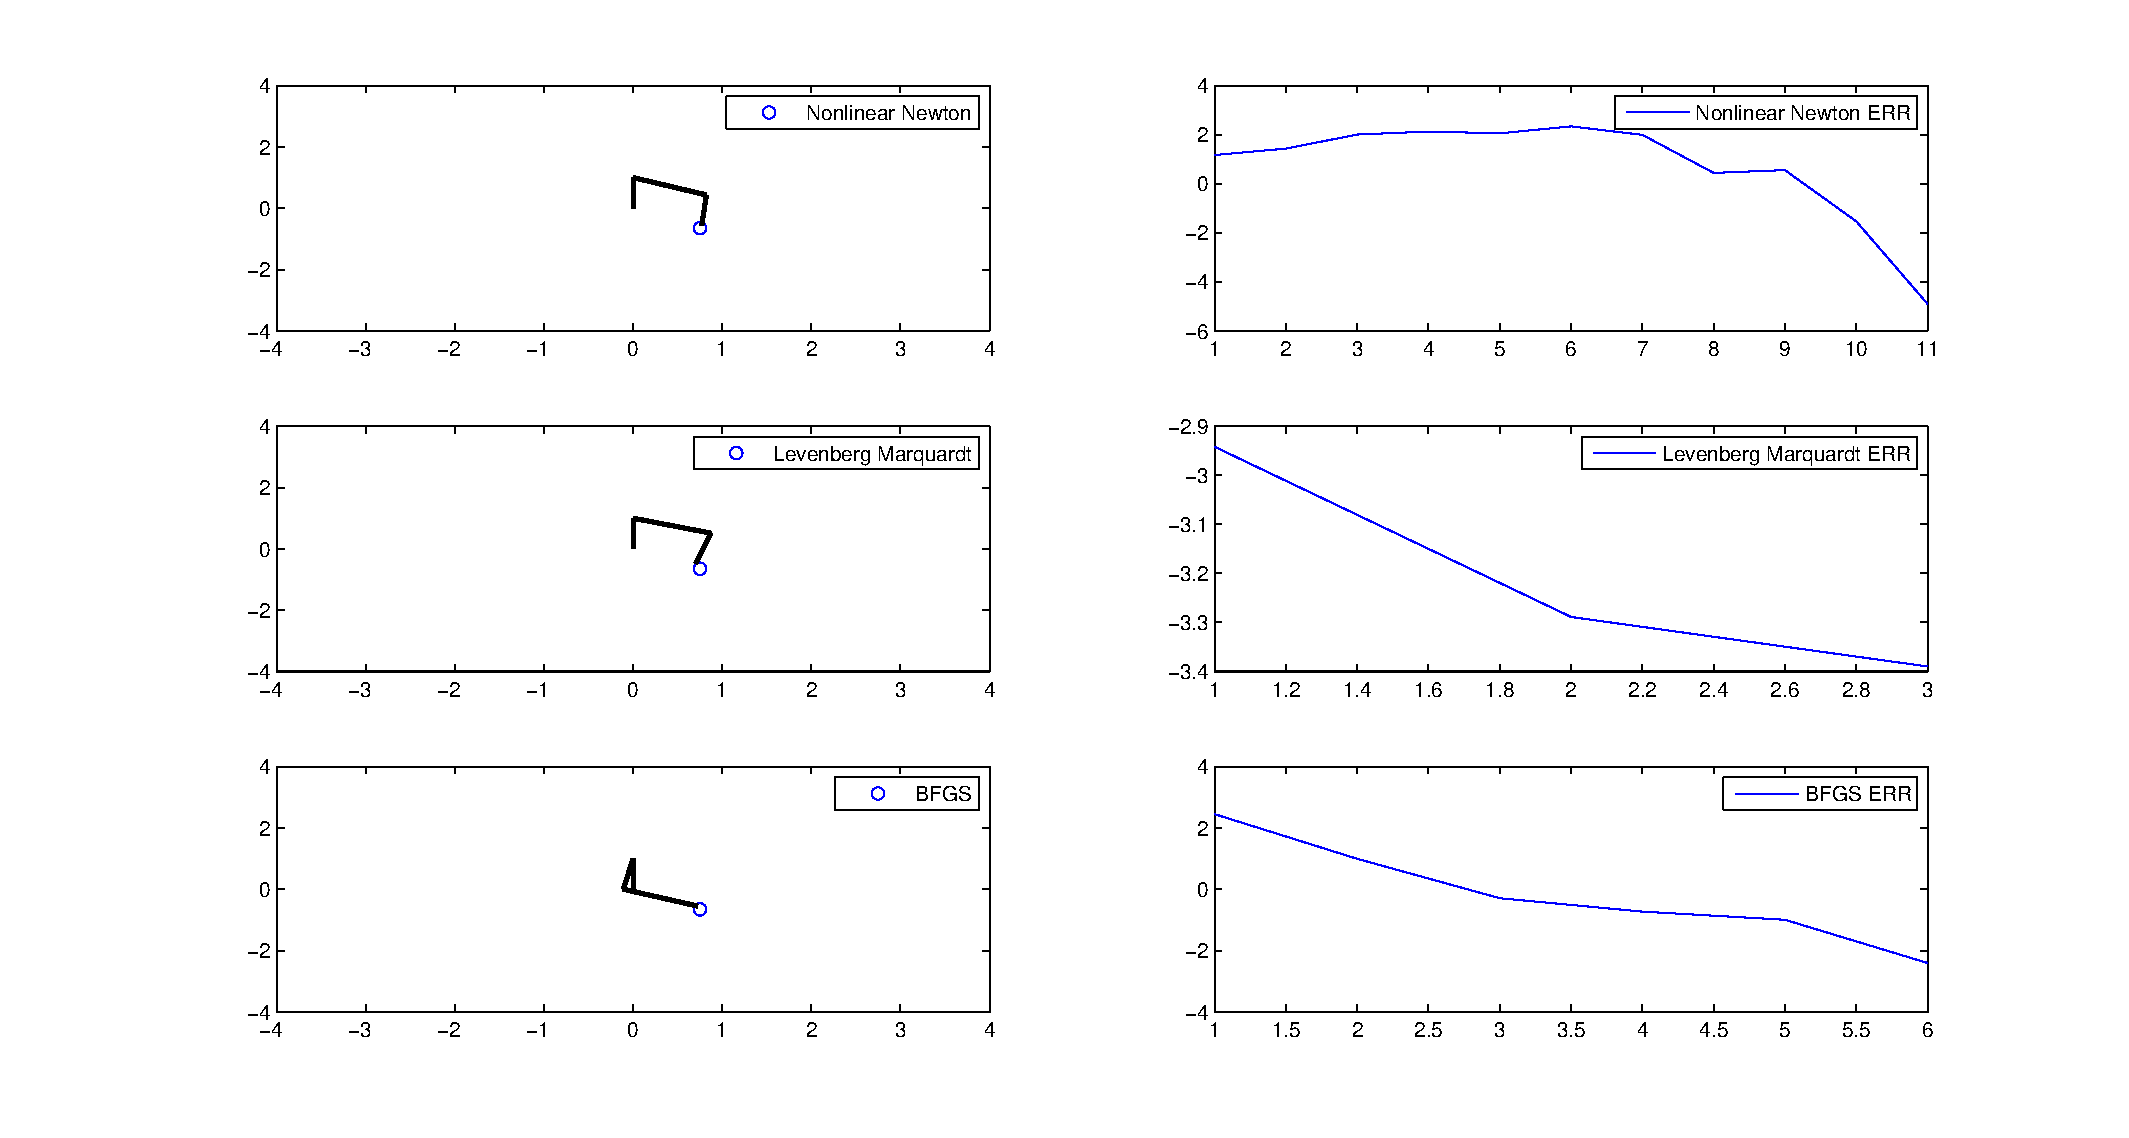
\includegraphics[width=\textwidth]{images/graph1.pdf}
This graph illustrates what I would have expected when I first started
to implement BFGS. It uses more iterations than Levenberg, but since
its iterations are cheaper it could very well be faster. In this case
methods finds a nice solution to the problem in few iterations.

\noindent
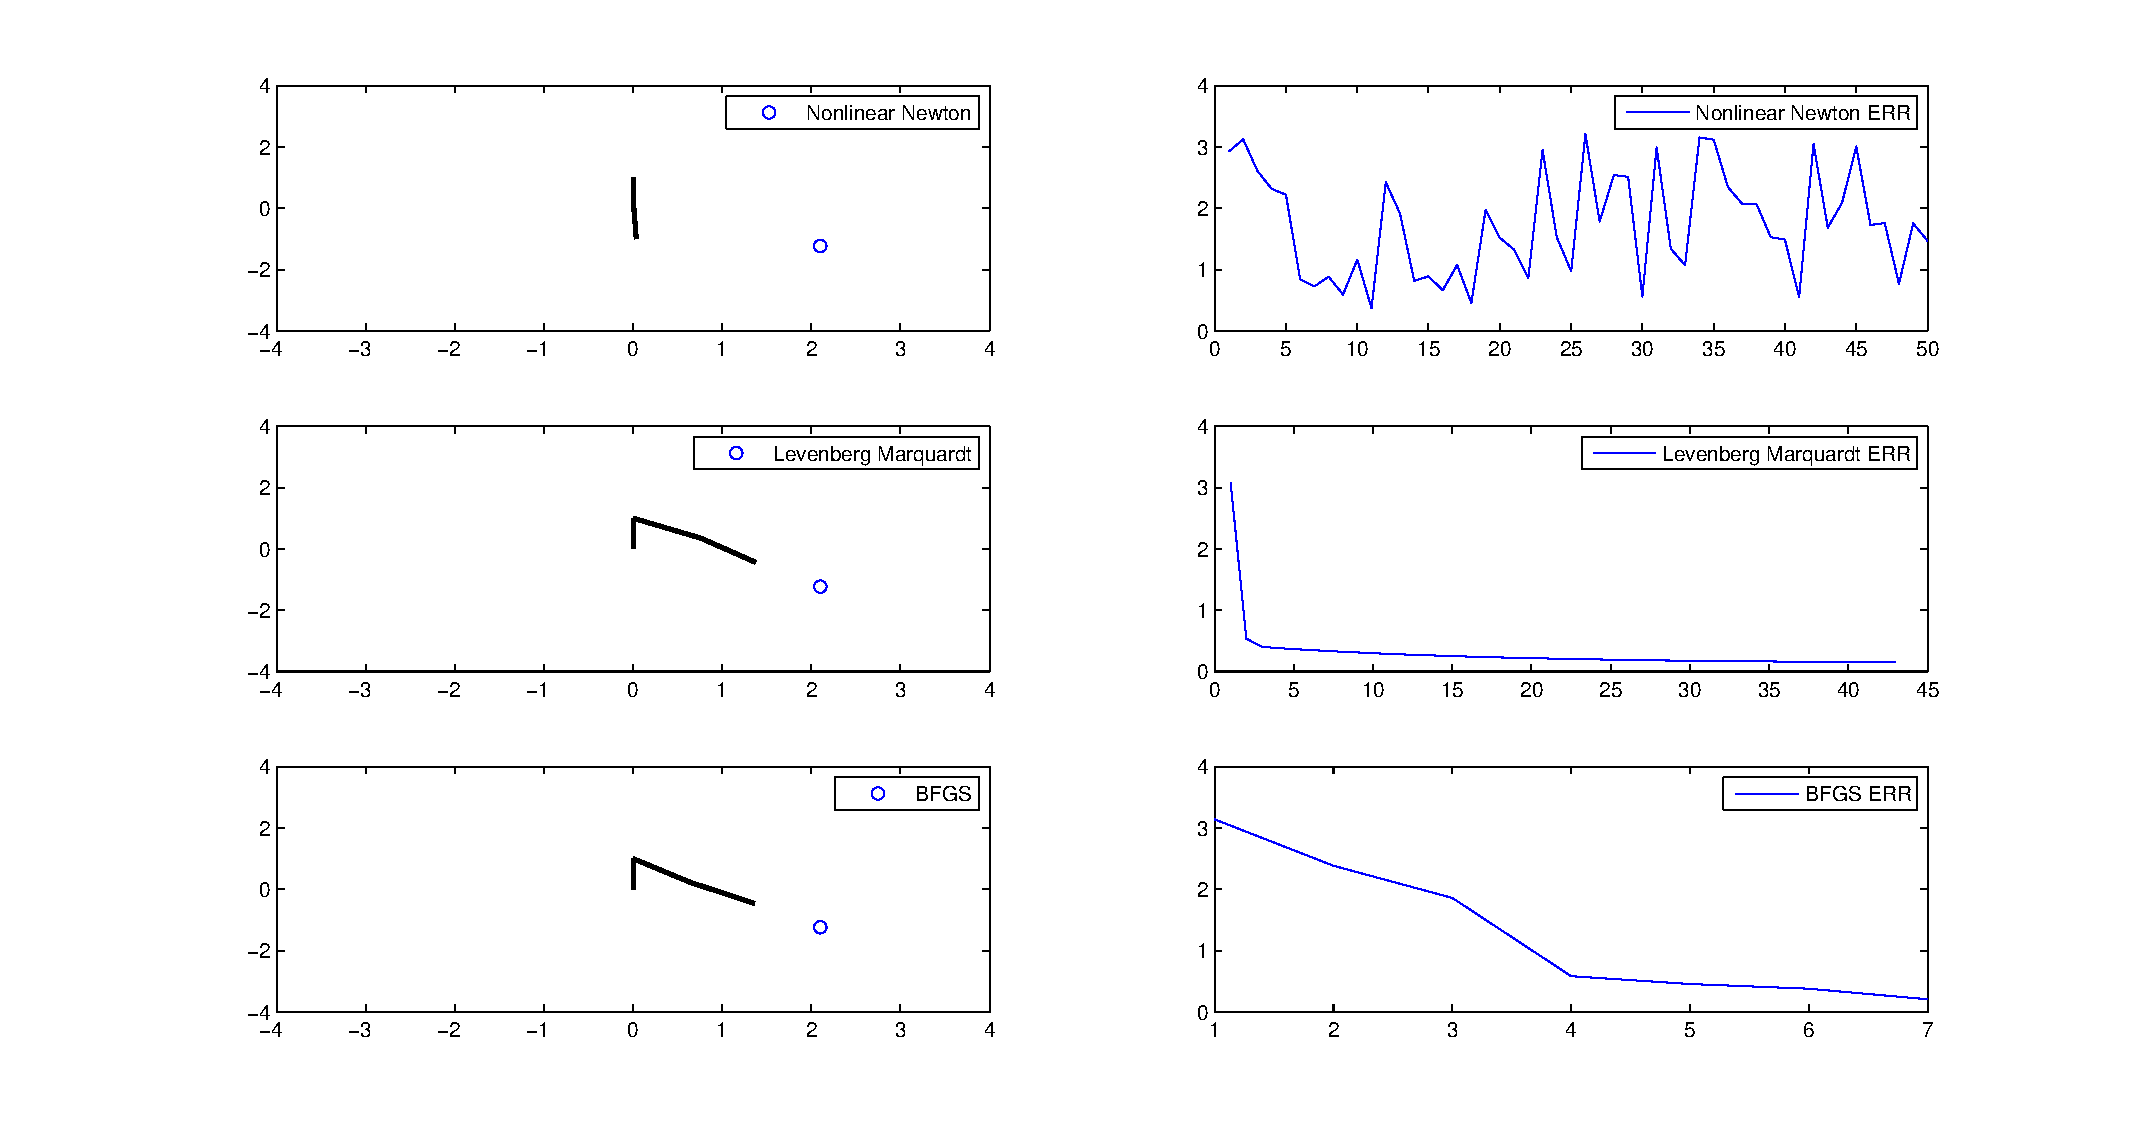
\includegraphics[width=\textwidth]{images/graph2.pdf}
In this case Newton's method fails to find an acceptable solution
while both Levenberg and BFGS finds one. This is because the selected
point is outside the reach of the ``arm''. I am not sure if I
understand why BFGS stops after just 7 iterations; far from the
goal. This should only happen if the gradient is very small.

\noindent
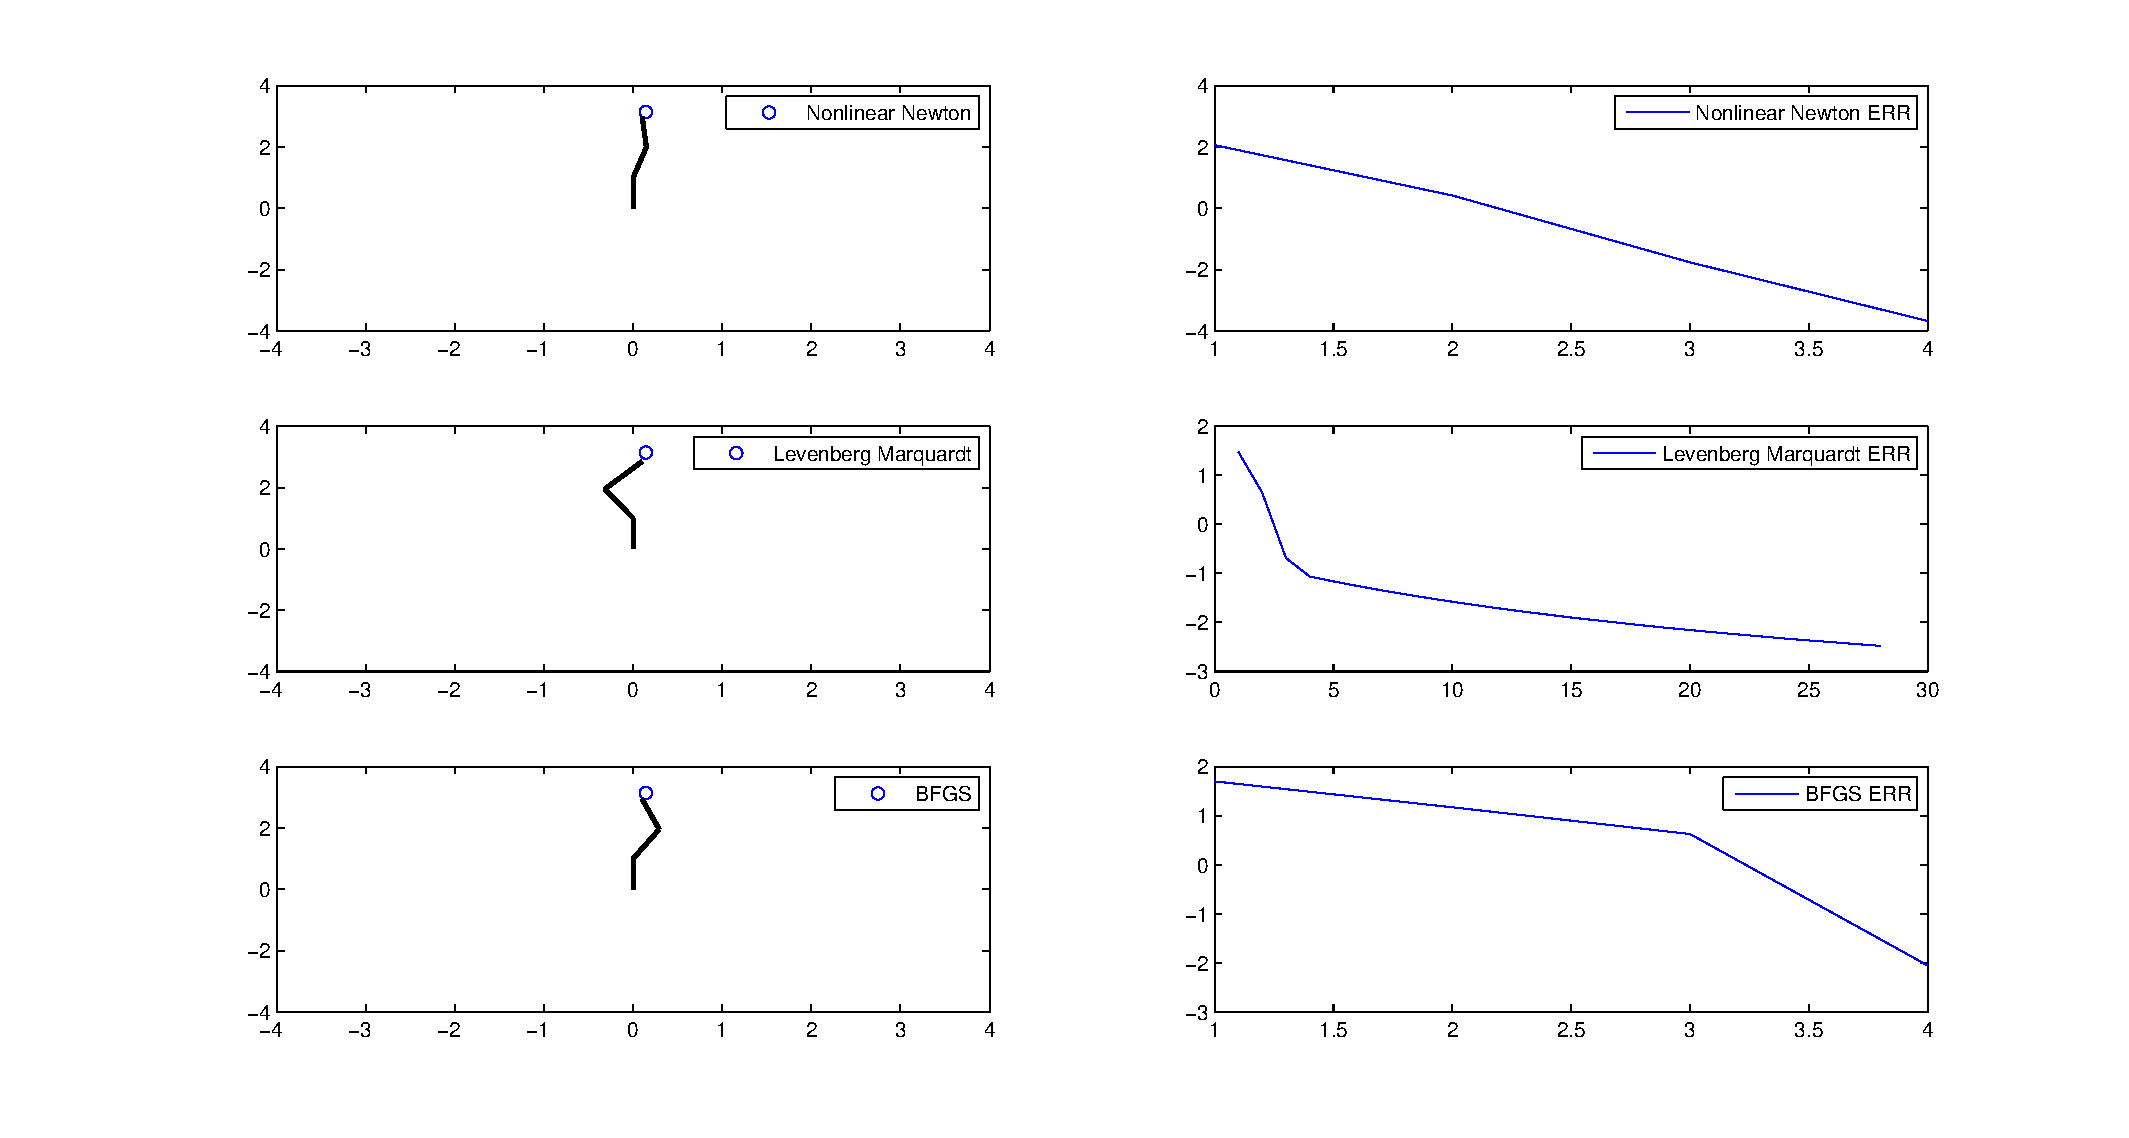
\includegraphics[width=\textwidth]{images/graph3.pdf}
Here Newton's method performs very well. Somehow this goal fits
perfectly with the process of Newton's method. BFGS keeps up using
just 4 iterations, however with a somewhat less confident
convergence. Levenberg doesn't perform well here with about 27
iterations.


\noindent
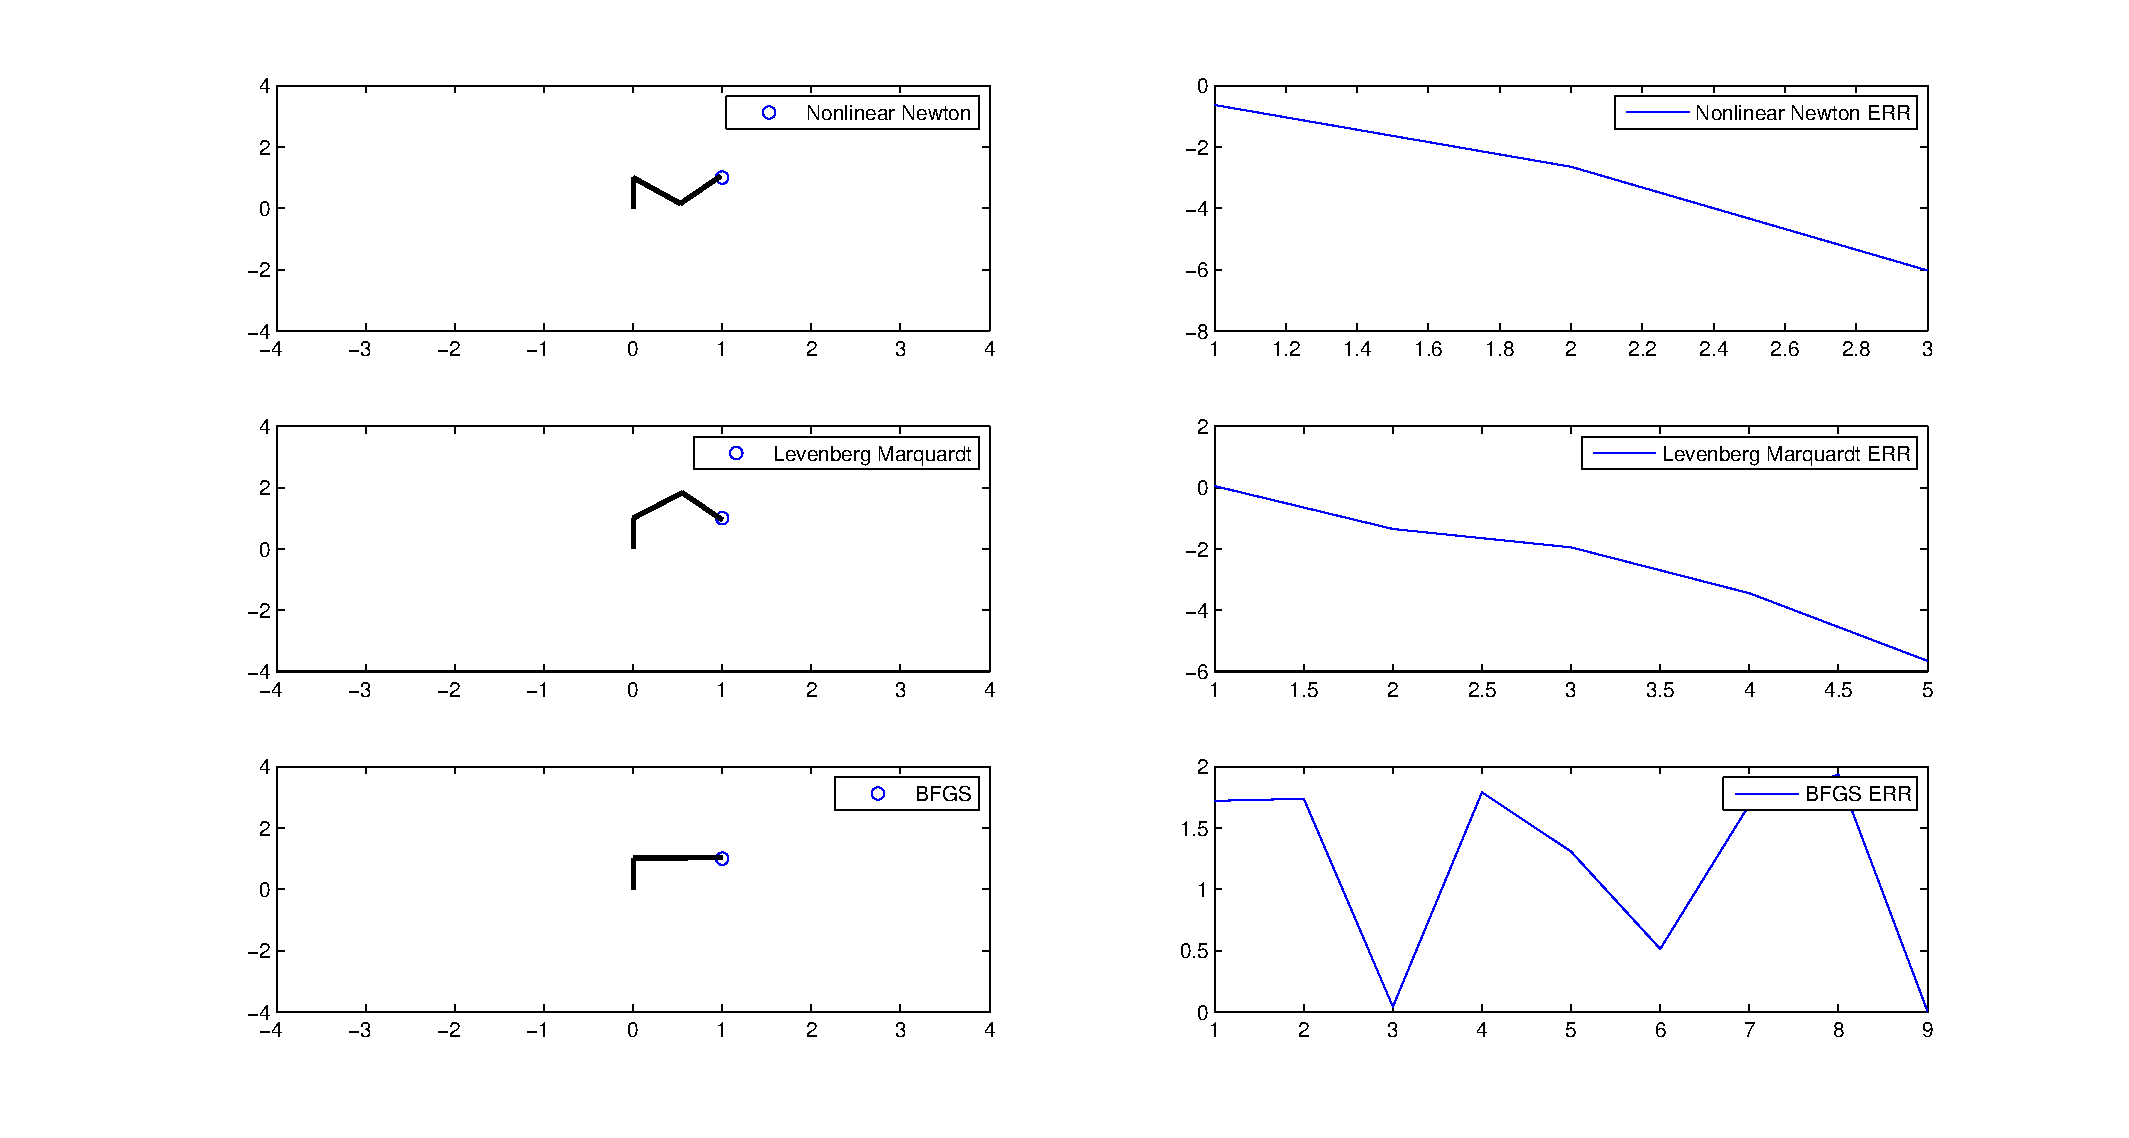
\includegraphics[width=\textwidth]{images/graph4.pdf}
I find this plot very interesting. All the methods manage to find a
solution in just few iterations, but look at BFGS's convergence graph.
It was very close to the goal after just 3 iterations, but then
something happened. What I think is, that $\alpha$ was chosen too
large. It jumped over the solution. This could happend if the
Armijo-condition could not be satisfied within the accepted size of
$\alpha$. In this case, the impementation takes a small step to ensure
movement to a new point, even though the step is up hill. Luckily
another solution was just around the corner at 9 iterations.


\section{Conclusion}
I have implemented the BFGS line-search method and compared this to
the previous implementations of the nonlinear Newton's method and
Leveberg-Marquardt.

With respect to the optimizations performed as part of the
verification the BFGS seems to perform better than the other
methods. It does not always use less iterations, but its iterations
are significantly faster to compute, since it avoids computation of
both the hessian and matrix inversion.

This one is for you Morten: The reason my results were imprecise was
that I had mistakingly computed an approximation of the Hessian - and
not its inverse. Fixing this gave a more precise approximation of the
inverse and hence more precise solutions with better convergence.



\end{document}

%%% Local Variables:
%%% mode: latex
%%% TeX-master: t
%%% End:
